\subsection{Problem}
\renewcommand{\theequation}{\theenumi}
\begin{enumerate}[label=\thesection.\arabic*.,ref=\thesection.\theenumi]
\numberwithin{equation}{enumi}

\item In $\triangle$ABC with vertices 
\begin{multline}
\vec{A} = \myvec{2\\3}\quad
\vec{B} = \myvec{4\\-1}\quad
\vec{C} = \myvec{1\\2}
\end{multline}
	Find the equation and the length of the altitude from vertex $\vec{A}$.
	The following python code computes the length of the altitude $\vec{AD}$ in Fig.\ref{fig:qtwo}.
	\begin{lstlisting}
	./codes/triangle/q2.py
	\end{lstlisting}
	
	\begin{figure}[!ht]
	\centering
	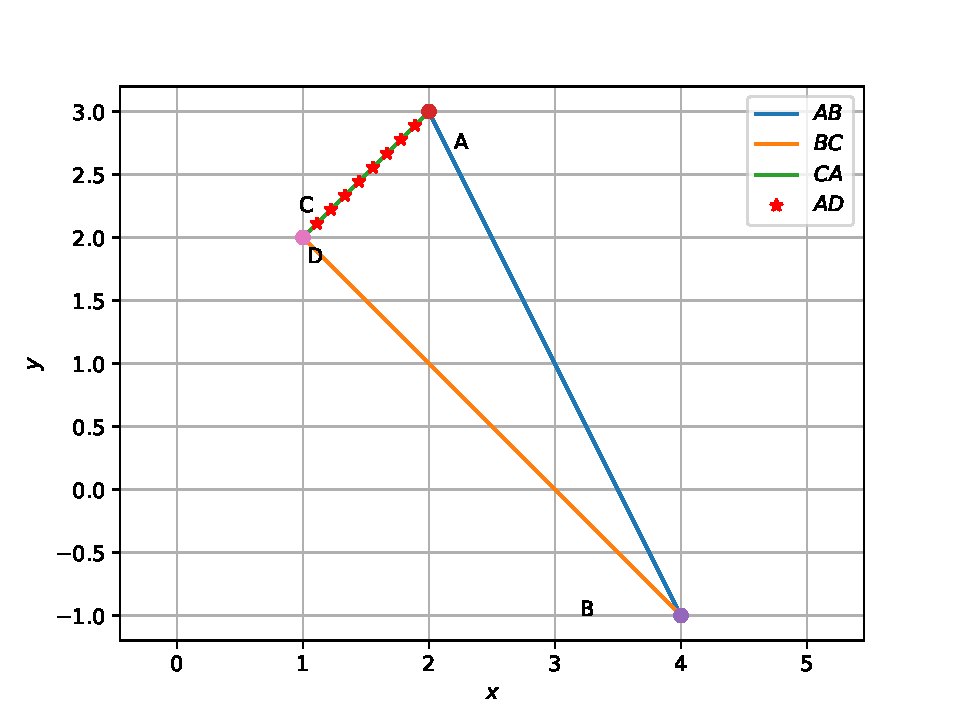
\includegraphics[width=\columnwidth]{./figs/triangle/q2.pdf}
	\caption{Triangle of Q.1.2.5}
	\label{fig:qtwo}	
	\end{figure}
	
	
	\solution Let the direction vector $\vec{m = B-C}$
	We define the normal vector
	\begin{align}
		\vec{n} = \myvec{0&1\\-1&0}\vec{m}
	\end{align}
	Equation of line $\vec{AD}$ is obtained as:
	\begin{align}
		\vec{m^Tx} = \vec{m^TA}
	\end{align}
	
	Equation of line $\vec{BC}$ is :
	\begin{align}
		\vec{n^Tx} = \vec{n^TB}
	\end{align}
	
	Since $\vec{D}$ is the intersection of lines $\vec{AD}$ and $\vec{BC}$ 
	\begin{multline}
		\myvec{\vec{m}&\vec{n}}^T \vec{D}= \myvec{\vec{m^TA}\\\vec{n^TB}}
		\\
	\text{which is solved to obtain the value of }\vec{D} = \myvec{1\\2}
	\end{multline}
	
	Therefore  The length of the altitude is obtained as $\norm{\vec{A-D}} = 1.414$
	
	
	
	
\end{enumerate}
